\documentclass[conference]{IEEEtran}
\IEEEoverridecommandlockouts
% The preceding line is only needed to identify funding in the first footnote. If that is unneeded, please comment it out.
\usepackage{cite}
\usepackage{url}
\usepackage{fancyvrb}
\usepackage[svgnames]{xcolor}
\usepackage{graphicx, float}
\usepackage{amsmath,amssymb,amsfonts}
\usepackage{algorithmic}
\usepackage{graphicx}
\usepackage{textcomp}
\usepackage{xcolor}

\graphicspath{{Figures/}}
\def\BibTeX{{\rm B\kern-.05em{\sc i\kern-.025em b}\kern-.08em
    T\kern-.1667em\lower.7ex\hbox{E}\kern-.125emX}}
\begin{document}

\title{Research Paper: Cyberattack Case Study \\CIS 3360-Security in Computing\\Fall 2025\\
{\footnotesize Instructor: Jie Lin, Ph.D.}
\thanks{}
}

\author{{ Derek Oliveira}\\
\IEEEauthorblockA{\textit{department of engineering and computer science} \\
Orlando, United States of America \\
de937084@ucf.edu}
}

\maketitle

\begin{abstract}
The SolarWinds cyber breach, revealed in December 2020, is one of the most significant cyber-espionage incidents in recent history. 
Through a complex supply chain compromise of SolarWinds’ Orion platform, the state-sponsored hacker group NOBELIUM gained ongoing and 
secret access to U.S. government agencies, corporations, and critical service providers. This paper looks at the historical background,
 motivations, and technical details of the attack that enabled persistent anonymous access to SolarWinds’ build environment, called SUNBURST.
  The breach not only penetrated high-level networks but also damaged global trust in software ecosystems. By examining NOBELIUM’s tactics and 
  the broad impacts of the intrusion, I argue that the SolarWinds incident serves as a wake-up call in cybersecurity. It reveals the vulnerability 
  of supply chains, shows the weaknesses of traditional defense methods, and points us toward new industry standards that shape the cybersecurity 
  landscape today.
\end{abstract}

\begin{IEEEkeywords}
SUNBURST, SolarWinds breach, supply chain attack, NOBELIUM, cyber espionage, CIA triad, Persistent access, critical infrastructure security
\end{IEEEkeywords}

\section{Introduction}

% Identify the attack, when/whom it affected, why it meets the significance 
% criteria, your thesis, and a brief roadmap.

On December 13, 2020, SolarWinds, a technology company from Texas that creates network monitoring and IT management software, announced what would 
become the most significant cyber intrusion in history. The breach targeted their Orion software, which is SolarWinds' main network monitoring platform.
 This platform is used by U.S. government agencies, defense contractors, Fortune 500 companies, and vital national service providers. The attackers, 
 later named NOBELIUM by Microsoft's Threat Intelligence Center (MSTIC), were identified as a state-sponsored group backed by Russia. As a result,
  NOBELIUM aimed for espionage instead of financial gain. 

SolarWinds itself wasn't the main target; instead, its compromised software supply chain served as the means for malicious code that entered its 
customers' networks undetected for over a year. Many exploits were used in this attack, but I will focus on the "SUNBURST" exploit for this research.

By the time the intrusion was discovered, NOBELIUM had secured their ongoing, unnoticed access to email servers, sensitive repositories, and classified 
communications for more than a year. This wasn't just a simple data breach. It was a careful and planned campaign of cyber-espionage that took advantage
 of trust to hide malicious intentions. The SolarWinds incident was seen as a major cyberattack, not only due to its size and complexity but also because
  of the national security threat it posed and the trust it undermined in global technology leaders, who monitor our interconnected world.

I believe that the SolarWinds breach marks a critical moment in cybersecurity. It showed the weaknesses in software supply chains, highlighted the flaws 
in existing detection systems, and prompted governments and companies to reconsider how resilient their networks are and how they can reorganize to lessen 
the impact of such breaches. To support this argument, I will first provide the historical background and motives of NOBELIUM, then look at the technical 
methods used in the SUNBURST intrusion, followed by an analysis of the attack's unique features, its wider geopolitical effects, and whether the attack 
strategies are still being used today. Finally, I will discuss the lessons learned and how this incident changed modern approaches to cyber defense.


\section{Background}
%History of Development (actor/group, prior incidents, sponsorship, timeline) 
%and Purpose & Motivation (financial, political, espionage, disruption).
\subsection{NOBELIUM}
NOBELIUM, previously known as APT29, UNC2452, Cozy Bear, Midnight Blizzard, and The Dukes, is a Russian-based threat actor 
identified by U.S. and European leaders as the foreign intelligence service of the Russian Federation\cite{Microdoft2024NOBELIUM}.
 NOBELIUM can be traced back to 2013, when European and American foreign ministries reported data breaches and theft of information. 
 This incident became known as "Operation Ghost."\cite{MITREFirstNOBELIUMAttack} NOBELIUM is recognized for manipulating trust within 
 security systems, falsifying digital certificates, impersonating IT managers, and distorting security protocols to achieve its objectives.
  These operations and tactics highlight NOBELIUM's focus on infiltrating high-value targets and gaining long-term access to sensitive information.

\subsection{History of Development}
The SolarWinds campaign unfolded over an extended timeline, as illustrated in Fig. \ref{fig:Timeline-of-Solorigate-attacks}. Initial 
reconnaissance and infiltration of SolarWinds’ infrastructure began as early as September 4, 2019, when NOBELIUM quietly embedded itself 
into the company’s software build process. By September 12, 2019, malicious test code had been injected into SolarWinds’ servers without
 detection, allowing the attackers to gather critical data and refine their ultimate payload, SUNBURST.\cite{MicrosoftDeepDiveSOLORIGATE}
\begin{figure}[H]
    \centering
    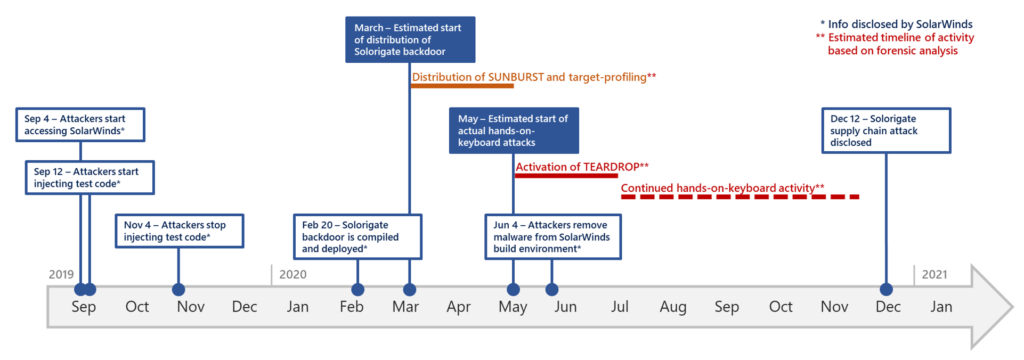
\includegraphics[width=3.4in]{Timeline-of-Solorigate-attacks.png}
    \caption{Image created by the MSTIC team on the timeline of events that led to the discovery of the SolarWinds
    breach.\\Source: \cite{MicrosoftDeepDiveSOLORIGATE} }
    \label{fig:Timeline-of-Solorigate-attacks}
\end{figure}

On February 20, 2020, NOBELIUM created a stable version of SUNBURST and released it in SolarWinds’ build environment. The malware was designed 
to stay hidden, waiting for real Orion software updates to be compiled before injecting its backdoor code. This meant that once the updates were 
sent out, thousands of unaware customers would install compromised versions of Orion. By March 2020, this supply-chain attack had effectively 
established hidden backdoors across SolarWinds’ global customer base.\cite{MicrosoftDeepDiveSOLORIGATE}

Two months later, NOBELIUM expanded its activities by launching TEARDROP, a custom loader for Cobalt Strikes, against specific high-value targets. 
This enabled the attackers to gain higher access, move laterally, and set up their true goals with minimal detection. On June 4, 2020, they eliminated 
all traces of the malware from SolarWinds’ build environment. This act made their presence even harder to detect and removed forensic evidence. At this 
point, no signs of compromise remained within SolarWinds’ infrastructure, leaving investigators with few leads.\cite{MicrosoftDeepDiveSOLORIGATE}

For months afterward, “hands-on-keyboard” activities continued as NOBELIUM carried out real-time surveillance, extracted sensitive documents, and stole 
credentials across compromised networks. Their secret campaign went mostly unnoticed until December 12, 2020, when SolarWinds publicly revealed the 
breach of its Orion software and the significant compromise of its customers’ systems.\cite{MicrosoftDeepDiveSOLORIGATE}



\subsection{Purpose and Motivation}
Unlike cybercriminal groups that aim mainly for financial gain, NOBELIUM's campaign was driven by political motives. 
Its goal was espionage, not profit. By taking advantage of SolarWinds' trusted software supply chain, the group gained hidden access to U.S. 
government agencies. This included the Department of Homeland Security, the Treasury Department, parts of the Pentagon, and major corporations 
in technology and critical infrastructure. The intelligence they collected had potential value for strategic leverage, diplomatic advantages, 
and competition in technology.

The reasons for the breach fit with Russia's larger geopolitical strategy of weakening adversaries, gathering intelligence, and showing power 
in the digital world. By compromising secure communications, source code repositories, and decision-making processes, NOBELIUM accessed state 
secrets and also damaged confidence in the security of the West’s digital infrastructure. This attack marks a clear shift from disruptive cyber 
incidents. It represents a long-term, secret infiltration campaign aimed at maximizing intelligence while keeping detection to a minimum.



\section{Analysis}
%Intended Usage Domain & Penetration Strategy 
%(industry/target environment, initial access, TTPs) 
%and Distinctive Features (innovations, what made it effective/different).
\subsection{Overview of SUNBURST (S0559)}
SUNBURST (MITRE S0559)\cite{MITRE2025SunburstS0559} is a trojanized component of SolarWinds' Orion platform that was compiled into
signed product updates and distributed to customers, it moved through Orion's build process as illustrated in figure \ref{fig:SUNBURSTPath}. Because 
the malicious code was delivered inside through vendor signed updates, it bypassed many integrity and whitelist checks
and achieved wide, trusted distribution. The implant combined application-layer mimicry, protocol obfuscation, and context-aware activation logic to 
remain dormant and undetected
until it found valuable execution environment.
\begin{figure}[H]
    \centering
    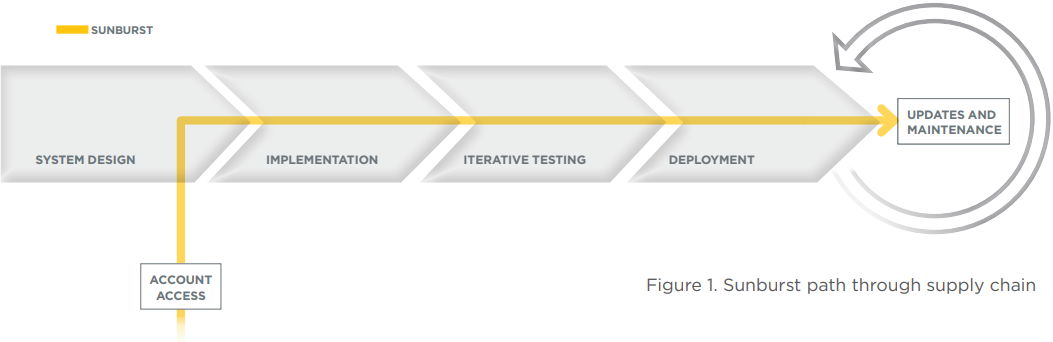
\includegraphics[width=3.4in]{SUNBURST-path.png}
    \caption{Source: \cite{BrokenTrustHerrEtAl} }
    \label{fig:SUNBURSTPath}
\end{figure}

\subsection{Intended Usage Domain and Penetration Strategy}
SUNBURST targeted the software supply chain rather than a particular target. It's vehicle was the Orion legitimate updates, which gave it reach into federal civilian agencies,
parts of the intelligence and defense communities, major tech firms, and critical infrastructure operators that installed Orion for network monitoring. Environments where trusted
vendor updates are accepted and administrators grant monitoring software broad visibility and privileges.
\subsubsection{Initial Access}
trojanized build artifact
\begin{itemize}
    \item Vector: Compromise of SolarWinds' CI/Build environment to insert malicious code into the Orion build through the masking of a legitimate dll file(SolarWinds.Orion.Core.BusinessLayer.dll).
    The malicious file was then digitally signed and released as part of a legitimate update.\cite{MicrosoftDeepDiveSOLORIGATE}
    \item Dormancy and environment checks: After installation, SUNBURST employed time delays, execution-context filtering, and logic to avoid activating in low value environments.
    It performed checks against its command and control(C2) routines, minimizing the risk of noisy execution that could trigger detection.\cite{MicrosoftDeepDiveSOLORIGATE}
    \item C2 communications: SUNBURST established covert C2 over common application protocols, mainly http, and through DNS techniques. Its C2 used obscured payloads, in the likes
    of base64 junk data, and dynamically resolved domains resembling trusted services, bypassing network signature detection and blending in with normal traffic.\cite{MicrosoftDeepDiveSOLORIGATE}
    \item Secondary payload staging: Once a high value target was identified, SUNBURST was a starting point for the delivery of the second payload, mainly TEARDROP or other cobalt strike loaders.
    This second stage had the attackers perform hands-on keyboard operations to harvest credentials, lateral movement, and data collection.\cite{MicrosoftDeepDiveSOLORIGATE}
    \item Persistence and cleanup: SUNBURST used standard persistence mechanisms and then later removed artifacts from the SolarWinds' build environment to delay incidence responses
    and forensic analysis \cite{MicrosoftDeepDiveSOLORIGATE}. SUNBURST also had the ability for remote writing and deleting of registry keys, it was observed stopping services by setting
    \fbox{/CurrentControlSet/services/*service name*/Start} registry entries to value 4\cite{MITRE2025SunburstS0559}. 
    \item Why it was so effective: Vendor signatures and normal updates processes caused endpoint and update-management systems to treat the payload as 'authentic' software
    rather than malicious code, completely skipping through the safety layer of hash based integrity checks. Covert C2 communications where established and hashed for dificult network signature detection\cite{MITRE2025SunburstS0559}.
    SUNBURST maintained a persistent foothold on SolarWinds' build environment and guaranteed its back door remained open throughout the duration of the operation, deleting itself from existance after cleaning 
    any artifacts left over from the attack.
\end{itemize}
\subsection{Distinctive Technical Features}
\begin{itemize}
    \item Exploitation of code provenance and trusted signing: SUNBURST's distribution inside legitimate signed binaries nullified at the time many traditional
    trust controls. The adversary weaponizes the very mechanisms that industry leaders rely on to verify software authenticity. This elevated a single compromise to a global vector of trust distribution.
    \item Protocol impersonation and C2 camouflage: SUNBURST mimicked legitimate Orion communications and used application layer behaviors to blend  C2 with normal monitoring traffic.
    The exploit's use of HTTP/DNS channels with encoded payloads and intermittent, low volume callbacks made detection using simple network indicators extremely difficult.
    \item Context aware activation: The artifact incorporated logic to delay activation and to selectively target environments and hosts, ensuring that the adversary only escalated activity
    where intelligence value justified increase risk. This surgical selectivity meant widespread infection did not equate to widespread exploitation, reducing the probability of early detection.
    \item Two stage model (stealthy loader + follow-on tooling): SUNBURST served as a stealthy, survivable loader. NOBELIUM followed up with custom
    loaders(TEARDROP/Cobalt Strike) to perform noisier operations once select targets were identified\cite{MicrosoftDeepDiveSOLORIGATE}. This separation
    of responsibilities amplified the campaign's effectiveness and allowed NOBELIUM to remain undetected for months.
    \item Operational trade craft: Documented behavior shows deliberate removal of artifacts from the build environment. Low noise hands-on-keyboard 
    operations in victims networks have been logged and analyzed. The combination of careful evidence cleanup and patient, long term
    surveillance that allowed for months of intelligence harvest without public detection, constituted into the hallmarks of state-level trade craft. 
\end{itemize}




\section*{Discussion}
% Active Descendants (whether methods persist/evolved), 
% full CIA triad impact, broader consequences, preventive and 
% punitive responses, lessons learned.

SUNBURST did more than steal secrets, it provided a playbook. The fundamental idea of subverting trusted vendor channels to deliver malicious code at
scale turned into a template for later actors. The method's potency relies on exploiting trust(signed updates, vendor attestation, and auto patching)
rather than a single technical vulnerability. In short, the technique persisted conceptually and evolved operationally. Attackers learned to be more
surgical, improving the camouflaged C2 as they went by with their surveillance. They mixed bespoke implants with commodity tooling so that each compromise
could be converted into a targeted intelligence operation. The legacy of SUNBURST is then twofold. An enduring template for high-stakes espionage and
a continuing arms race that forces both vendor and consumer practices to change.
\subsection{Full CIA Triad Impact}
\subsubsection*{Confidentiality (C)}
SUNBURST inflicted severe confidentiality breaches. By inserting a persistent stealthy backdoor into Orion, NOBELIUM gained access to email systems,
source-code repositories, secret documents, and internal communications. The theft of classified information without detection was the attack's primary
goal.
\subsubsection*{Integrity (I)}
Integrity was undermined at a foundational level. NOBELIUM altered the source of software artifacts, turning vendor signed binaries into vehicles
for malicious code. This corrupted the very notion of "trust" and damaged confidence in update streams and signed mechanisms. In victim networks,
attackers manipulated configuration, inserted backdoors, and in some observed instances altered logs or other forensic data, actions that complicated
accurate reconstruction of events.
\subsubsection*{Availability (A)}
Although the SolarWinds campaign primarily sought espionage rather than widespread disruption, availability was indirectly threatened. The compromise
exposed privileged access paths that could be repurposed to disrupt services, derail incident response, or create conditions for DOS(Denial of Service)
or destructive attacks. Moreover, the domino effect due to the compromise of trust produced real availability costs for organizations that had to take
their systems offline or restrict operations to remediate risk.

\subsection{Broader consequences}
SUNBURST exposed systematic weaknesses in assumptions about software provenance and the limits or perimeter defenses. Organizations discovered
that signature-based update verification could be insufficient against an adversary that controls code at the source. The incident accelerated
interest in supply-chain hardening practices and in runtime behavioral and telemetry analysis that can detect malicious activity despite valid 
signatures.\\
The breach generated tangible economic costs as well. It reshaped procurement and vendor-risk calculus, buyers increasingly demanded stronger
contractual cybersecurity assurance, breach disclosure terms where made into existence, and a push for more transparent vendor build practices.\\
At a strategic level, the campaign deepened mistrust between nation-states and highlighted cyber espionage as a tool for geopolitical leverage.
The operation demonstrated the asymmetry of cyber power, disproportionate access to another state's secrets without any brute force. This reality
intensified calls for international cyber norms, attribution mechanisms, and coordinated defensive postures among allied nations.\\
Regulators and policymakers used the incident to justify stricter disclosure rules, supply-chain audits, and incident reporting requirements\cite{NCSC2021FurtherTTPsSVR}.
The incident also energized discussions about sanctions and legal consequences for state-linked actors, and it spurred legal scrutiny of vendor liability
and responsibilities to secure their build processes.
\subsection{Preventive and Punitive Responses}
    The sequence of events that unfolded after the SolarWinds incident, as shown in figure \ref{fig:AfterMathTimeLine}, teaches us that preventive responses must operate on
    multiple layers to close the pathways SUNBURST exploited. At the technical level, organizations and governments
    must emphasize policy reforms and shifts in industry practices that explicitly work to reduce complexity and produce greater speed and agility. To
    maximize resilience, the government must work with industries to prioritize programs dedicated for cybersecurity and the education of good practices
    not just for professionals in the field, but to its users as well. Governments must also harness the power of the open source communities to 
    make linchpin tech more defensible. Furthermore, any shift in policy/protocol must guarantee a more adaptive system is left behind. A system where 
    every failure does not constitute to a complete overhaul of the entire system, but incremental iterations on imperfections for scalability.
    \begin{figure}[H]
        \centering
        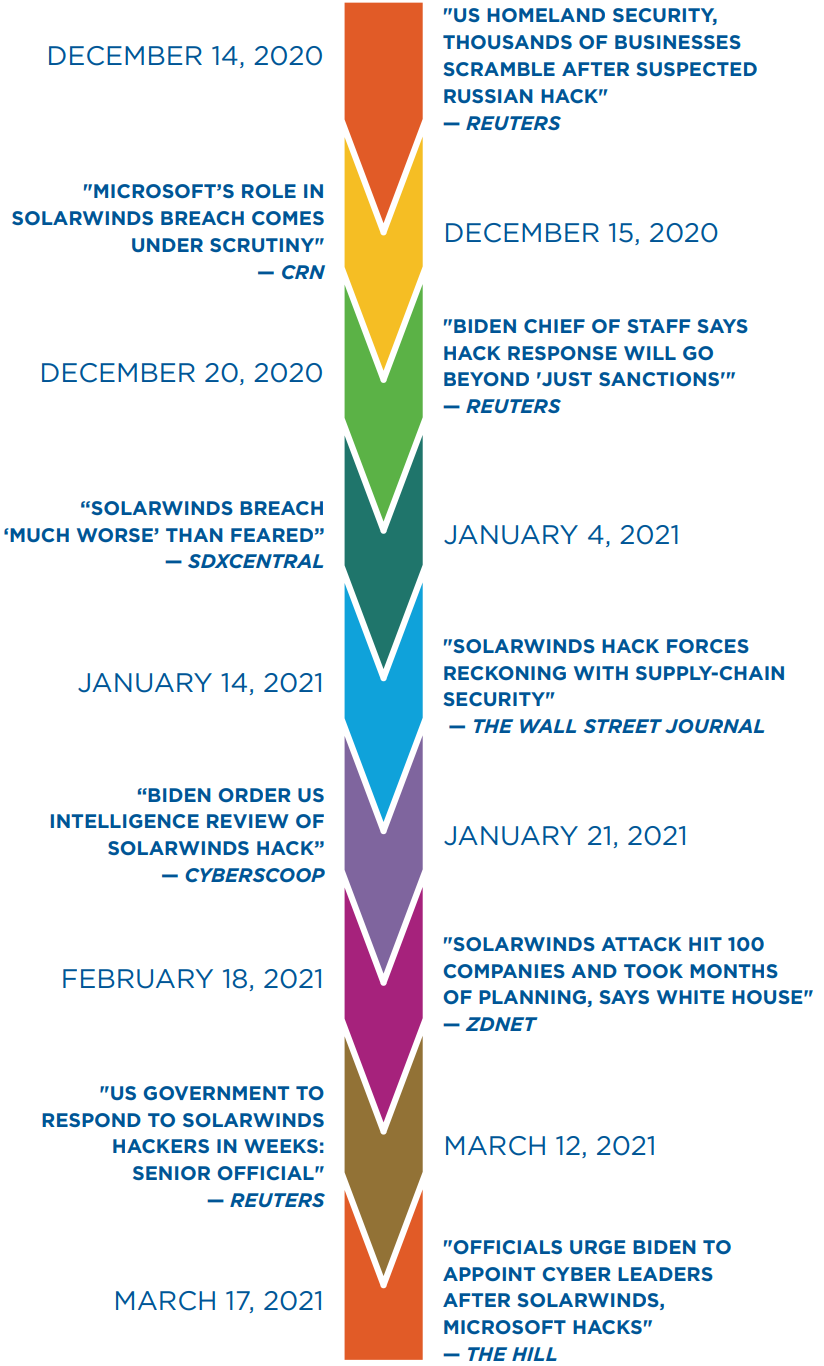
\includegraphics[width=3.4in]{AfterMath-Timeline.png}
        \caption{Source: \cite{BrokenTrustHerrEtAl} }
        \label{fig:AfterMathTimeLine}
    \end{figure}
The response from the U.S. Government on the SolarWinds incident was a direct message that the west was not going to take
this breach lightly. The Cybersecurity and Infrastructure Security Agency (CISA), Federal Bureau of Investigation (FBI), and the
Office of the Director of National Intelligence (ODNI), with support from the National Security Agency (NSA),
cooperated to form two Cyber Unified Coordination Groups (UCG), one for the SolarWinds incident and one for the
Microsoft exchange incident\cite{GAOSolarWindsExchange}. Together with corporations, the two UCGs worked diligently to come up with adequate responses
and advisories from the lessons learned in this incident. From December 13th, 2020, through July 19, 2021, UCGs and their
respective government agencies issued Emergency Directives, Advisories, information on the Advanced Persistent Threat (APT),
Private Industry Notifications (PIN), Tools for unusual malicious activity, and malware analysis reports
\cite{GAOSolarWindsExchange}. On April 9th, 2021 enough information was uncovered from the incident that the Department
of Justice (DOJ) obtained a warrant to remove web shells from U.S. based victim servers that had been compromised.\\
On April 15th, 2021, the U.S. Department of the Treasury released to the press sweeping new sanctions targeting Russian actors related to
the attackers of the SolarWinds' incident. As a result of the sanctions, all property and interest in property
belonging to designated persons that are located in the United States or under the control of U.S. persons
where to be frozen and reported to OFAC. Under the "50 percent rule," any entity that is owned, directly or indirectly, 50 percent or more by one
or more blocked persons was also automatically blocked. Unless specifically authorized by OFAC through a general or
special license, U.S. persons are broadly prohibited from conducting transactions involving blocked persons or their property. This 
prohibition extends to the provision or receive of funds, goods, services, effectively cutting sanctioned individuals
and entities off from the U.S. financial systems and most commercial activities\cite{DepartmentOfTreasuryResponse}. Although not very effective
to a Country that already was heavily sanctions, most punitive responses where put in place for symbolism; The U.S. will not tolerate any intrusion into
its systems and critical networks.\\ 
In a tit-for-tat response, the Russian Foreign Ministry expelled 10 American foreign diplomats from the country, barred entry to eight current and former
U.S. Officials, including the U.S. attorney general, the heads of the FBI, NSA, DHS, FBP, the national security advisor, former
CIA director, and the domestic policy council director.\cite{TheGuardianRussiaExpelsDiplomats}
    \subsection{Lessons Learned}
    The "Broken Trust" report by T. Herr, W. Loomis, et al\cite{BrokenTrustHerrEtAl}, emphasizes that the incident was less an isolated
    technical failure but a strategic breakdown in how the U.S. organizes its cybersecurity posture and risk management.
    The authors argue, with success, that the crisis exposed a mismatch between fast evolving adversaries
    and defensive institutions that are slow, overburdened, and fragmented. The conventional approach of layering
    more controls, more standards, and more committees risk reinforcing complexity without resolving the underlying problem.
    Instead, public and private sectors must embrace a concept the authors call "persistent flow." Persistent flow simply means the posture
    private and public sectors must take to quickly and ruthlessly prioritize risk, act decisively at critical points, and synchronize efforts
    across institutions.\\
    Another central lesson learned is the technical vulnerabilities exploited by SUNBURST were not novel or wholly
    unpredictable. They were variations on supply-chain attacks that had occurred before. The attack on SolarWinds'
    supply chain amplified the existing structural weaknesses in software ecosystems, build systems, and procurement
    practices. What made SUNBURST exceptional was its integration with cloud identity services and its ability
    to reach deeply into both on-premises and cloud environments. That being said, I agree with the authors of
    "Broken Trust" when they advise that the betterment of our security will not come from simply bettering our current 
    code, but a complete systemic redesign. Emphasize on making core vendor platforms more defensible, reducing reliance
    on fragile cloud primitives, and aligning procurement, regulations, and industry to better reflect realities of adversarial
    competition.

\section{Conclusion}
%key findings, recommendations, future implications, and limitations.
The SolarWinds breach, carried out through the SUNBURST exploit, clearly showed how the very systems meant to protect and simplify 
modern networks can be turned into tools for destruction. By penetrating SolarWinds’ software supply chain and embedding harmful 
code into trusted Orion updates, NOBELIUM gained ongoing, hidden access to some of the most sensitive networks worldwide. This 
operation shattered the belief that digital signatures and vendor updates provide unbreakable guarantees of authenticity, revealing 
deep flaws in the global software ecosystem. The result was a serious compromise of U.S. government agencies and companies, along 
with a loss of trust in the reliability of the digital infrastructure that supports national security and international trade.

The lessons from SUNBURST go far beyond just this one attack. The incident highlighted that state-sponsored groups will keep evolving, 
improving their skills in mixing stealth with accuracy, and using trust relationships to their advantage. We need to implement preventive 
measures along with punitive actions like sanctions and joint diplomatic efforts to make these operations more costly. In the end, SolarWinds 
served as a wake-up call that resilience, not invulnerability, should be the main goal of cybersecurity strategy. The future of defense depends 
on flexible, systemic redesign. Only by understanding these lessons can governments and industries hope to resist the next wave of supply-chain 
attacks and maintain trust in the digital foundations of our modern society.

\section*{Citations}


\begin{thebibliography}{}
\bibitem{Microdoft2024NOBELIUM} Microsoft, ``Nation State Actors Midnight Blizzard,'' \emph{Microsoft Security Insider}, Jan. 25, 2024. [Online]. Available: \url{https://www.microsoft.com/en-us/security/security-insider/threat-landscape/midnight-blizzard}. [Accessed: Sept. 29, 2025].
\bibitem{MITREFirstNOBELIUMAttack} MITRE, ``Operation Ghost (Campaign C0023),'' \emph{MITRE ATT\&CK}. [Online]. Available: \url{https://attack.mitre.org/campaigns/C0023/}. [Accessed: Sept. 29, 2025].
\bibitem{MITRE2025SunburstS0559} MITRE, ``SUNBURST (Software S0559),'' \emph{MITRE ATT\&CK}. [Online]. Available: \url{https://attack.mitre.org/software/S0559/}. [Accessed: Oct. 1, 2025].
\bibitem{MicrosoftDeepDiveSOLORIGATE} Microsoft Cyber Defense Operations Center and Microsoft Threat Intelligence, ``Deep Dive into the Solorigate Second-Stage Activation: From SUNBURST to TEARDROP and Raindrop,'' \emph{Microsoft Security Blog}, Jan. 20, 2021. [Online]. Available: \url{https://www.microsoft.com/en-us/security/blog/2021/01/20/deep-dive-into-the-solorigate-second-stage-activation-from-sunburst-to-teardrop-and-raindrop/}. [Accessed: Sept. 29, 2025].
\bibitem{CoreTech2022Motivations} CoreTech Staff, ``6 Motivations of Cyber Criminals,'' \emph{CoreTech Blog}, Mar. 3, 2022. [Online]. Available: \url{https://www.coretech.us/blog/6-motivations-of-cyber-criminals}. [Accessed: Sept. 29, 2025].
\bibitem{HakalaMelnychuk2021RussiaCyberStrategy} J. Hakala and J. Melnychuk, *Russia’s Strategy in Cyberspace*, NATO Strategic Communications Centre of Excellence, Riga, Latvia, Jun. 2021. [Online]. Available: \url{https://stratcomcoe.org/cuploads/pfiles/Nato-Cyber-Report_11-06-2021-4f4ce.pdf}. [Accessed: Sept. 29, 2025].
\bibitem{NCSC2021FurtherTTPsSVR} National Cyber Security Centre (UK), ``Advisory: Further TTPs Associated with SVR Cyber Actors,'' May 2021. [Online]. Available: \url{https://www.ncsc.gov.uk/files/Advisory-further-TTPs-associated-with-SVR-cyber-actors.pdf}. [Accessed: Sept. 30, 2025].
\bibitem{BrokenTrustHerrEtAl} T. Herr, W. Loomis, E. Schroeder, S. Scott, S. Handler, and T. Zuo, *Broken Trust: Lessons from Sunburst*, Atlantic Council, Scowcroft Center / Cyber Statecraft Initiative, Mar. 2021. [Online]. Available: \url{https://www.atlanticcouncil.org/wp-content/uploads/2021/03/BROKEN-TRUST.pdf}. [Accessed: Sept. 30, 2025].
\bibitem{GAOSolarWindsExchange} U.S. Government Accountability Office, *Cybersecurity: Federal Response to SolarWinds and Microsoft Exchange Incidents*, GAO Report No. GAO-22-104746, Jan. 2022. [Online]. Available: \url{https://www.gao.gov/assets/gao-22-104746.pdf}. [Accessed: Sept. 30, 2025].
\bibitem{DepartmentOfTreasuryResponse} U.S. Department of the Treasury, *Treasury Sanctions Russia with Sweeping New Sanctions Authrity*, April 15, 2021. Available: \url{https://home.treasury.gov/news/press-releases/jy0127}. [Accessed: Oct. 01, 2025]
\bibitem{TheGuardianRussiaExpelsDiplomats} The Guardian, ``Russia expels 10 US diplomats as part of retaliation for sanctions,'' Apr. 16, 2021. [Online]. Available: \url{https://www.theguardian.com/world/2021/apr/16/russia-expels-10-us-diplomats-etaliation-sanctions}. [Accessed: Sept. 30, 2025].
\end{thebibliography}
\vspace{12pt}

\end{document}
